\documentclass{article}
\usepackage[lmargin=2.54cm, rmargin=2.54cm,tmargin=2.54cm,bmargin=2.54cm]{geometry}
\usepackage{doc}
\usepackage{graphicx}
\usepackage{indentfirst}
\usepackage{setspace}

\title{Homework 3}
\author{Anthony Menjivar}
\date{}
\begin{document}
\maketitle
\section{Java Bozosort}
\begin{center}
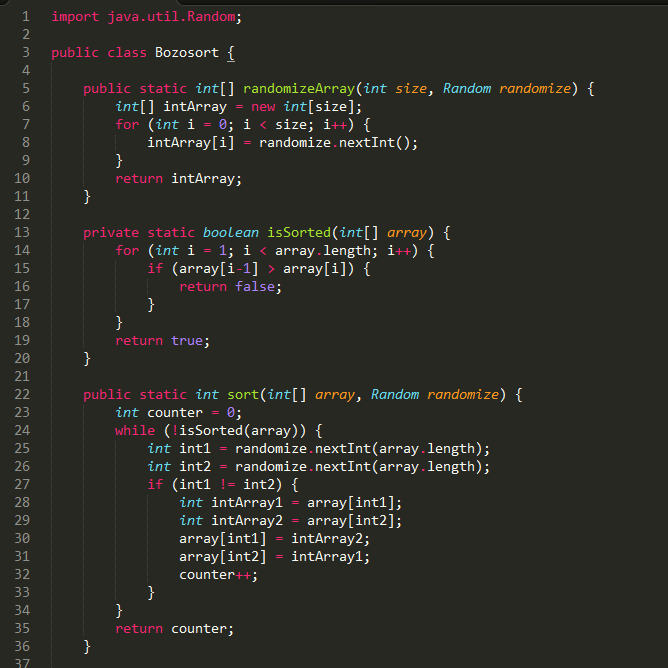
\includegraphics{Bozosort1.png}
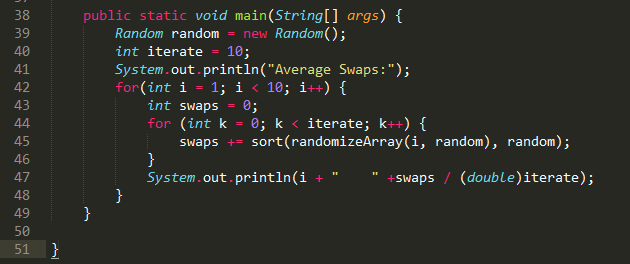
\includegraphics{Bozosort2.png}
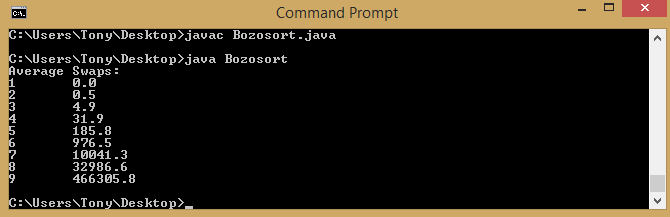
\includegraphics{BozosortTable.png}
\end{center}

\section{Java Autokey Vigenere Cipher}
\begin{center}
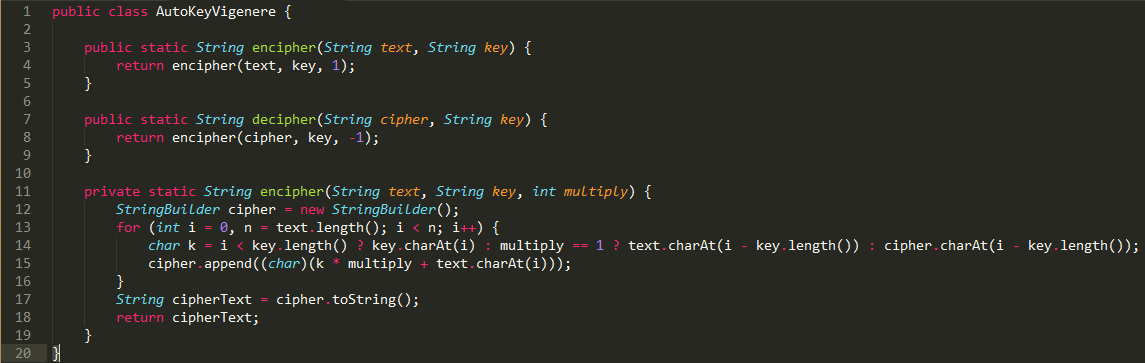
\includegraphics[scale=0.5]{AutoKeyVigenere.png}
\end{center}

\section{Monoalphabetic Substitution Cipher Plaintext}
UIQLDEVORHIWLTQTOKMQMWROUOQQMQLKIQWQVIEWRDQTLEQMWRWXFTWHTOA

DMRDQIOKWXMAOHMRMRHQVOQWLTAOMRQODPMDQWMRDQTLEQOEWAFLQITBVOQ

QWKWUIQLDEWREIRQTOQITOQVITWRIJFUOMRMRHQWVLAORSIMRHDBVOQBIBO

RQOEWAFLQITQWKW

\vspace{5mm}

LETUSCHANGEOURTRADITIONALATTITUDETOTHECONSTRUCTIONOFPROGRAM

SINSTEADOFIMAGININGTHATOURMAINTASKISTOINSTRUCTACOMPUTERWHAT

TODOLETUSCONCENTRATERATHERONEXPLAININGTOHUMANBEINGSWHATWEWA

NTACOMPUTERTODO

\section{bifid Algorithm Decryption}
TWBTLLAEPODTUBTWBTLTDLDDVSNNHEETLSKDDSIFGIIMWLYDKDDSPHBPQKOFHMDLSKRS

\vspace{5mm}

COMPUTERSCIENCEISNOMOREABOUTCOMPUTERSTHANASTRONOMYISABOUTTELESCOPESS

\section{Private Key}
If someone's RSA public key is (729880581317, 5), what is her private key?

\vspace{5mm}

private key is $(N,d)$

$N=729880581317$ $N=pq$ 

$p=822893$ $q=886969$

$(p-1)(q-1)=729878871456$

$d=5InverseMod(729878871456) $

Private Key = $(729880581317, 583903097165)$



\section{Problem 1.45}
\subsection{a}
We would want digital signature schemes because they can be used to authenticate the sender's identity and to make sure that the message has not been altered by a third party during communication.
\subsection{b}
$((N, e), M^{d}, M)$

$(M^{d})^{e}$ mod $N$ = $(M^{e})^{d}$ mod $N$ = $M$ mod $N$ = $M$

\vspace{2mm}

If someone were able to sign given only $(N,e)$, they would be able to exponentiate by $d$ mod $N$, which allows decryption, contradicting RSA security. So if RSA is secure, this scheme is also secure.

\subsection{c}
$p = 137$ $q = 71$ $e = 99$

$N$ = $pq$ = $9727$ and $m_{1}^{d}$

Extended Euclid:

$d$ = $6539$
\subsection{d}
RSA key = (17, 391)

Factor 391 to $17 * 23$

$\Phi(391)$ = $16 * 22$ = $352$

Using Extended Euclid:
$d$ = $(e)^{-1}$ $mod$ $352$ = $145$

\vspace{2mm}

Check:
$145 * 17$ = $2465$ = $1$ $mod$ $352$

\section{Problem 1.46}
\subsection{a}
The message sent by Alice to Bob is the encrypted message $M^{e}$ $mod$ $N$. With this, if Bob agreed to sign anything he is asked to with his private key, Eve will obtain $(M^{e})^{d}$ $mod$ $N$ = $M$.
\subsection{b}
Eve can ask Bob to sign $M^{e} * k^{e}$ $mod$ $N$, where Eve picks k coprime to N at random.By using Extended Euclid Even can find M. This way Bob's signature is distributed in the same way over all numbers inverted mod N.

\section{Problem 2.4}
\subsection{a}
Master Theorem:

$a = 5, b = 2, d = 1$

$a > b^{d}$

Run time:

$O(n^{log_{b}a})$ =  $O(n^{log_{2}5})$ = $O(n^{2.33})$

\subsection{b}
T(n) = 2T(n - 1) + C, for a constant C.

C$\Sigma_{i=0}^{n-1}$ $2^{i}$ + $2^{n}T(0)$ = $O(2^{n})$

\subsection{c}
Master Theorem:

$a =9, b = 3, d = 2$

$a = b^{d}$

$O(n^{d}logn)$ = $O(n^{2}logn)$

I would choose this one.

\section{Problem 2.12}
Each time the function is called it prints out one line and calls the same function on half the size of the input. This means that the number of printed lines is:

$P(n)$ = $2P(\frac{n}{2}) + 1$

\vspace{2mm}

Using Master Theorem:

$P(n) = \Theta(n)$

\section{Problem 2.23}
\subsection{a}
In splitting the two arrays, we have A1 and A2. If A has a majority element, that element must also be a majority of A1 or A2 or both. To find the majority element, we recursively compute the majority elements of A1 and A2 and check whether any of these is a mahority element of A. The running time is $T(n)$ = $2T(\frac{n}{2}) + O(n)$ = $O(nlogn)$

\subsection{b}
There are at most n/2 elements because at least one element in each pair is discarded. If the remaining elements have a majority element then there exist x of them within the elements appearing at least n/4 times. Therefore, x must have been paired up with itself in at least n/4 pairs, meaning thatqq there are at least n/2 of x. The running time for this is $T(n)$ = $T(\frac{n}{2}) + O(n)$. Meaning $T(n)$ = $O(n)$ 

\section{Problem 3.2 (a)}
$A \rightarrow B \rightarrow C \rightarrow D \rightarrow H \rightarrow G \rightarrow F \rightarrow E$

\section{Problem 3.8}
\subsection{a}
Let (directed) graph G = (V,E).

Triple nodes (a0, a1, a2)

Container sizes: C0 = 10, C1 = 7, C2 = 4

ai is the actual contents in the ith container. 

$0 \leq ai \leq Si$ for i = 0, 1, 2 and at any given node a0 + a1 + a2 = 11. An edge between two nodes (a0, a1, a2) and (b0, b1, b2) exists if: (1) the two nodes differ in two coordinates and (2) if i, j are coordinates they differ in, then either ai = 0, or aj = 0 or ai = Si or aj = Sj.
\subsection{b}
Depth First Search Algorithm

\subsection{c}
On depth 6 on the depth first tree, the node (2, 7, 2) is reached which is the answer.

\end{document}
